%!TEX root = ../../Main.tex
\graphicspath{{Chapters/Test/}}
%-------------------------------------------------------------------------------


\section{Test}

\subsection{Matlab simulering}

Efter den teoretiske undersøgelse, vil vi i dette afsnit udvikle og vise en simuleret version af vores filter, hvor der er taget udgangspunkt i Teori afsnittet. Da vi tager udgangspunkt i teoriafsnittet starter vi med at vise hvordan vi har implementeret vores filter. 

\begin{lstlisting}
%Create LMS FIR filter
my = 0.01; % some number 0.01
W = zeros(1,256);

for n = 1:length(d) %run every sample 
    yn = 0;
    for m = 1:length(W) %make new filteret sample 
        if n > m
            yn = yn + fixed32(W(m)*noise(n-m));
        end
    end
    y(n) = yn;
    e(n) = d(n) - y(n);
    for m = 1:length(W) %make new koefficient  
        if n > m
            W(m) = W(m) + fixed32(my*noise(n-m)*e(n));
        end
    end
end
\end{lstlisting}

Først i filteret vælger vi en my, som ift til teori afsnittet bestemmer hvor hurtig filteret er. I dette eksempel bruger vi en værdi som er testet frem til at have et god forhold mellem hastighed og settling time. Herefter bestemmes hvor mange koefficienter filteret skal have. Vi har valgt et forholdsvis højt tal, da vi simulerer. Dette vil ikke nødvendigvis være muligt på Cross-core. \\

Igennem genereringen af filteret laves der 3 forloop. Et som kører hver sample igennem, et som laver det filtrede nye sample, og et som opdaterer koefficinterne ift tilbagekoblingen. \\
De nye filter koefficienter bliver herved opdateret til det ønskede filter, hvor e(n) bliver fejlen ift figur \ref{fig:LMS_filter}, som er det talesignal der ønskes. \\
Koden er bygget op sådan at vi kører en fixed16 og fixed32, for at simulere det bedst muligt ift blackfin. Fixed16 svarer til fixed point 1.15 og fixed32 til fixed point 1.31. 
\\
Dette giver os et filter som fungerer efter hensigten. Først testes der med 3 sinus toner, som ligger indover et tale signal, disse 3 toner skal derved gerne blive filtreret gennem filteret. 
\newpage
\subsubsection{Første test}
Den første test der blev udført var så simpel som mulig. I forsøget generes et talesignal med 3 sinustoner indover. 
Figur \ref{fig:Filter_time} viser signalet som bliver filtreret i tidsdomænet. Her er det værd at observerer settling tiden på filteret som ses i y(n). Denne settling tid vil kunne gøres mindre ved at justere på my. Der er valgt til opgaven her at teste med 0.01 my. 
\begin{figure}[H]
	\centering
	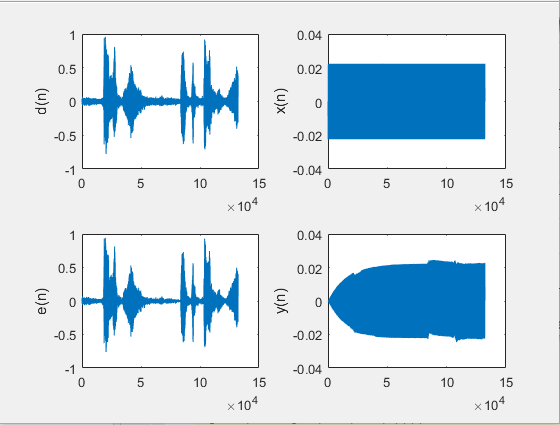
\includegraphics[width = 400pt]{Img/Filter_time}
	\caption{LMS filter i tid (3 sinus toner)}
	\label{fig:Filter_time}
\end{figure}
\newpage
Herefter vises på figur \ref{fig:Filter_Freq} signalet i frekvens domænet, her ses hvordan filteret filtrere den fejl som skabes fra, og derved skaber et signal e(n), som er talesignalet uden sinus tonerne. 

\begin{figure}[H]
	\centering
	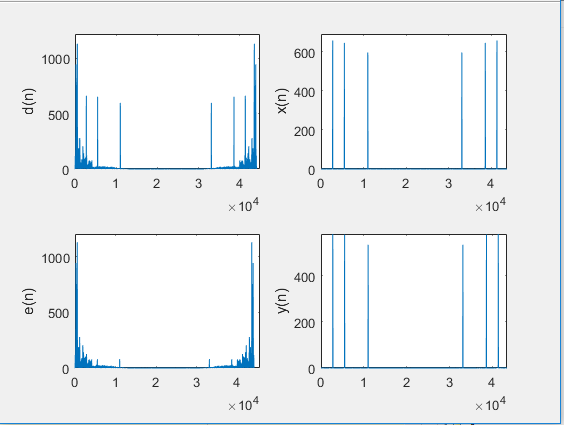
\includegraphics[width = 400pt]{Img/Filter_Freq}
	\caption{LMS filter i frekvens (3 sinus toner)}
	\label{fig:Filter_Freq}
\end{figure}
\newpage
Ved at kigge på selve filteret ses at filteret (figur \ref{fig:Filter}) skaber et filter som kune lukker de 3 sinus toner igennem, hvilket er hensigten. Dette signal bliver så fratrukket det endelige samlede signal, for at få en error som er det endelige e(n). 
\begin{figure}[H]
	\centering
	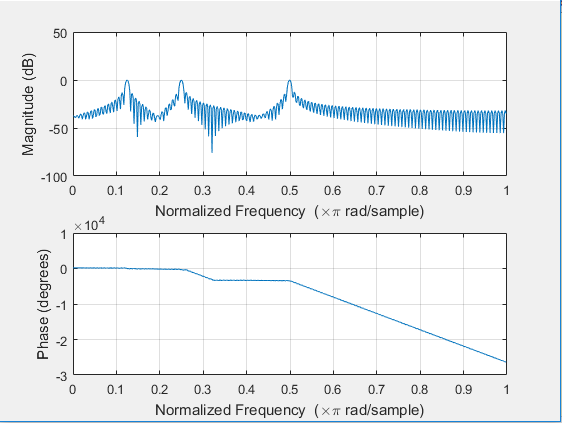
\includegraphics[width = 400pt]{Img/Filter}
	\caption{LMS filter(3 sinus toner)}
	\label{fig:Filter}
\end{figure}
\newpage
\subsubsection{Anden test}
Første test var i den nemme og simple ende, da vi kun skulle filtrere rene toner fra, vil der i anden test forsøges at filtere en foodprocessor som bekrevet i indledningen. Denne opgave en del mere udfordrende for filteret da den nu skal filtrere på mange toner og ikke kune 3, samtidig med den skal lade nogle bestemte toner gå igennem, som kommer fra talesignalet. \\
På figur \ref{fig:Filter_time_food}, ses nu det endelige produkt i tidsdomænet, der ses her en kraftig filtrering af signalet fra d(n) til e(n). Igen ser vi også en y(n) der har en settling time, inden filteret begynder at virke efter hensigten. 

\begin{figure}[H]
	\centering
	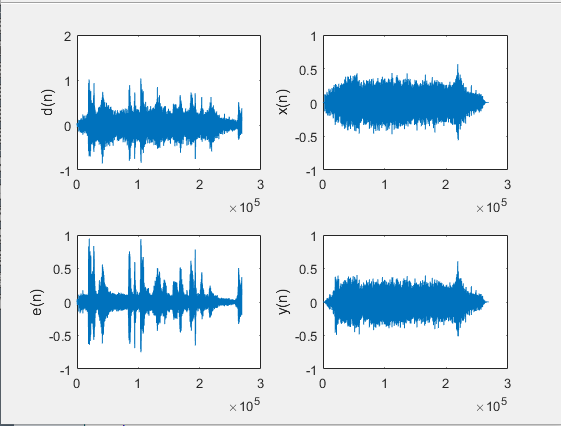
\includegraphics[width = 400pt]{Img/Filter_time_food}
	\caption{LMS filter i tid (food processor)}
	\label{fig:Filter_time_food}
\end{figure}
\newpage

Herefter tager vi et blik på frekvens donænet som viser lidt det samme billede som tidsdomænet, at LMS filteret filtrerer kraftigt fra d(n) til e(n), dette kommer af at foodprocessoren er indeholder mange lydfrekvenser. Hvis vi kigger lidt på figur \ref{fig:Filter_Freq_food}, og figur \ref{fig:Filter_food}, kan man nærstudere figur \ref{fig:Filter_food}, og se at filteret fungerer bedst når frekvenserne er udenfor talefrekvenserne, dette betyder også at filteret ikke prøve at filtrere støj fra som ligger i tale signalet, dette kan vi se fra figur \ref{fig:Filter_food}.

\begin{figure}[H]
	\centering
	\includegraphics[width = 400pt]{Img/Filter_Freq_food}
	\caption{LMS filter i frekvens (food processor)}
	\label{fig:Filter_Freq_food}
\end{figure}
\newpage

\begin{figure}[H]
	\centering
	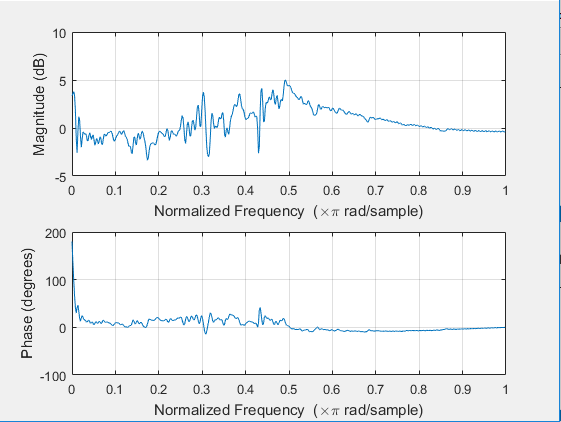
\includegraphics[width = 400pt]{Img/Filter_food}
	\caption{LMS filter(food processor)}
	\label{fig:Filter_food}
\end{figure}

\subsection{Cross-core}
\subsubsection{Overordnet}
Gruppen har valgt at lave test ud fra funktionalitet frem for use cases, da mange af use casene ikke vil godkendes, og derfor giver en forklaring af testene mere mening. 
 
\subsubsection{Visuel test}
Cross-core er et IDE, som kan programmere software over på blackfin proccesoren. Herigennem er der lavet embedded software, som styre forbindelserne på blackfin, samtidig med at vi udfører projektets funktionalitet. Igennem undervisnignen er der blevet henvist til signal proccesering framework, som også gøres brug af i denne opgave. 

Gennem denne test var der flere ting som udfordrede funktionaliteten , og sammenligningsgrundlaget ift matlab simuleringen. 
Da det nemmeste at sammenligne med er grafer og figurer, blev vi nød til at udskrive txt filer fra blackfin, som udskrev hver sample. Da blackfin har et begrænset memory, kunne vi dog kun have 1024 sample gemt, hvilket er et meget kort lydsignal. Dette var især en ulempe, da matlab modellen var bygget op af lydsignaler med en længde på 268723 samples. Dette gør en signifikant forskel. 
Hvis vi kigger på figur \ref{fig:Blackfin}, ser vi den realiserede proces med 3 toner, som også blev brugt i matlab modellen. Dette er valgt da det visuelt er meget nemmere at se på en graf frem for støj fra en food processor.
Hvis der sammnelignes med de første 1024 samples i matlab figur \ref{fig:Blackfin_simulering}, ser vi at matlab ikke filtrerer sinus tonerne fra som ved realiseringen på blackfin. Det skal med at skaleringen af tidssignalerne fra blackfin og matlab, ikke er den samme, dette skyldes fixedpoint, og at en txt fil kun kan have integer værdier. Det har dog ingen indflydelse på resultaterne, da skaleringen er den samme. Ydermere er der også ændret i koden, så første værdi er 1 og ikke 0, mere om det emne i diskussionen. 
\begin{figure}[H]
	\centering
	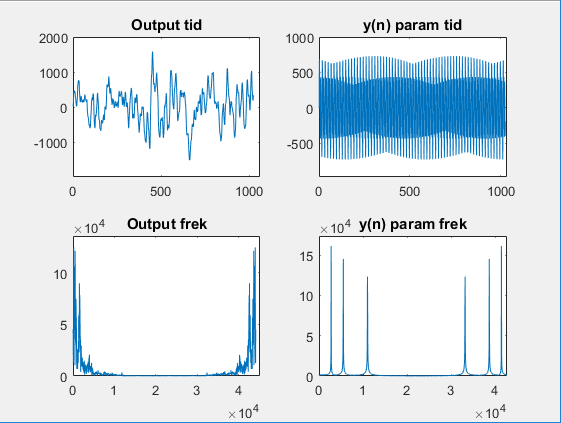
\includegraphics[width = 400pt]{Img/Blackfin}
	\caption{LMS filter implementeret på Blackfin}
	\label{fig:Blackfin}
\end{figure}

\begin{figure}[H]
	\centering
	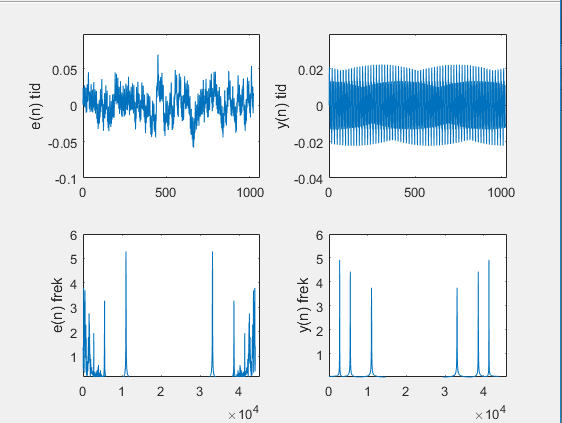
\includegraphics[width = 400pt]{Img/Blackfin_simulering}
	\caption{Simulering af figur \ref{fig:Blackfin} i matlab}
	\label{fig:Blackfin_simulering}
\end{figure}
\newpage
Hvis vi kigger nærmere på matlab simlueringen, af de samme signal og samme antal samples, undrer gruppen sig over hvordan det kan være at  matlab modellen bliver markant anderledes, og ikke ser ud til at virke efter hensigten. Dette kommer især til udtryk hvis vi kigger på figur \ref{fig:Tjek_af_frek}, hvor vi ser at frekvensen fra y(n) burde bliver trukket fra d(n), det ser dog ikke ud til at virke efter hensigten. Dette emne vil kort blive taget op i diskussionen igen. 
\begin{figure}[H]
	\centering
	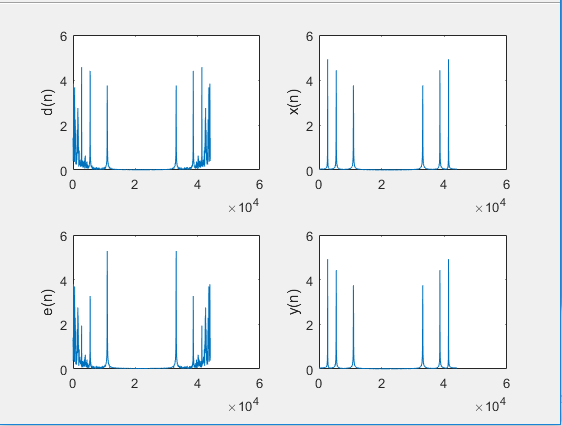
\includegraphics[width = 400pt]{Img/Tjek_af_frek}
	\caption{Fejl fra matlab filter}
	\label{fig:Tjek_af_frek}
\end{figure}

\subsubsection{Audio Test}
Gruppen har gennem testen lavet en audio test, hvor både sinus toner så vel som food processoren er blevet testet. 
Produktet og derved lyden virker til en vis grad igennem blackfin processoren. Hvis der sendes 3 sinus toner som både støj og implementeret i talesignalet, opleves at sinus tonerne fjernes, dog tilføres en "klik" lyd, som vil forsøges forklaret i diskusionen. Hvis vi derimod sender food processoren ind som støj og implementerer det i talesignal, bliver lyden forvrænget og filtrering af fejlen har ikke den ønskede funktionalitet ift at fjerne støjen. Dette vil igen blive diskuteret i diskussionen. 